\documentclass[10pt, compress]{beamer}

% Tema de la presentación
\usetheme[usetitleprogressbar, usetotalslideindicator]{m}

% Tabla de contenidos precedida de ∙
\setbeamertemplate{section in toc}{%
    ∙  \inserttocsection \par}

% Mejora de las tablas
\usepackage{booktabs}

% Inclusión de gráficos
\graphicspath{{./graphics/}{./graphics/screenshots/}}

% Extensiones de gráficos
\DeclareGraphicsExtensions{.pdf,.jpeg,.jpg,.png}

% Renderizado de la fecha
\usepgfplotslibrary{dateplot}

% Título
\title{Interfaz web para la gestión de sondas de red de altas prestaciones}
% Subtítulo
\subtitle{Trabajo de Fin de Grado}
% Fecha
\date{Junio 2015}
% Autor
\author{Juan Sidrach de Cardona Mora}
% Tutor
\newcommand{\tutor}{Sergio López Buedo}
% Logo Grupo de investigación
\newcommand{\logoResearchGroup}{Logo_hpcn}
% Logo Facultad
\newcommand{\logoFaculty}{Logo_EPS}
% Logo Universidad
\newcommand{\logoUniversity}{Logo_UAM}
% Grupo de investigación (comentado, mejor el logo)
% \institute{High-Performance Computing and Networking}

% Contenido
\begin{document}

% Portada
\maketitle

% Tabla de Contenidos
\begin{frame}{Tabla de Contenidos}
  \tableofcontents
\end{frame}

% Introducción
\chapter{Introducción}

Este Trabajo de Fin de Grado, realizado en colaboración con el grupo de investigación \textit{High-Performance Computing and Networking (HPCN)}, tiene como propósito el desarrollo de una interfaz web para la gestión de sondas de red de altas prestaciones.
En los siguientes apartados se explican la motivación y los objetivos principales del mismo, sucedidos de una descripción de la estructura del resto de la memoria.

\section{Motivación}

Una sonda de red es un dispositivo capaz de capturar tráfico de red (sonda pasiva) o de inyectarlo (sonda activa).
Este dispositivo puede ser algo tan sencillo como un ordenador convencional, en el cual se ha instalado una tarjeta \textit{Ethernet} estándar o una tarjeta a medida basada en \gls{FPGA}.
La aplicación a desarrollar se basará en una sonda de este último tipo~\cite{jfzazo}.

Hasta ahora, la única posibilidad existente es interaccionar con esta sonda desde la línea de comandos, lo que dificulta su gestión para personas sin conocimientos previos de la misma.
Otra dificultad en el control de la sonda es que existen numerosos aspectos relacionados con su funcionamiento que se manejan de forma externa, tales como el almacenamiento, clasificación y gestión de las \glspl{traza}.

Surge entonces la necesidad de una simplificación en el manejo de la sonda, que permita a usuarios no avanzados su utilización.
Para ello, se desarrollará una interfaz gráfica basada en tecnologías web, que facilitará conocer y manejar el estado de la sonda. Además, permitirá administrar otros aspectos del sistema, como los mencionados anteriormente.

\section{Objetivos}

Los objetivos principales planteados en este Trabajo de Fin de Grado son los siguientes:

\begin{itemize}
  \item Desarrollar una interfaz web que permita la gestión de una sonda de red de altas prestaciones.
  Esta interfaz permitirá, de manera visual, conocer el estado actual de la sonda de red y configurarla para reproducir o capturar tráfico de red.
  Además, la interfaz web permitirá gestionar las \glspl{traza} capturadas con la sonda mecionada.
  Se pretende así facilitar el control de todos los componentes que intervienen en la captura y reproducción de tráfico de red, y que no sea necesario conocer previamente el funcionamiento interno de la sonda para poder manejarla y experimentar con ella.

  \item Monitorizar el estado del servidor al que está conectada la sonda de red de altas prestaciones.
  Para ello, la aplicación mostrará al usuario estadísticas sobre el servidor relevantes en este contexto.
  Por una parte, se podrá conocer el espacio de almacenamiento disponible para guardar \glspl{traza}, para que el usuario pueda liberar espacio es caso de ser necesario, y prevenir así que la sonda deje de poder capturar tráfico de red.
  Por otro lado, si el sistema de archivos en que se almacenan las \glspl{traza} capturadas con la sonda está sobre un \gls{RAID}, se podrá conocer la velocidad de escritura global del sistema y de cada uno de los discos que integran el \gls{RAID}, ya que es un factor que puede limitar el rendimiento de la sonda.

  \item Registrar estadísticas sobre el uso de la aplicación, lo que ayudará a localizar y solucionar errores internos.
  Adicionalmente, se podrán analizar estos registros para conocer el grado de utilización de la sonda por diferentes usuarios, y plantearse entonces cómo optimizar el tiempo necesario para realizar las tareas más frecuentes.
\end{itemize}

\section{Estructura del documento}

En el capítulo~\ref{cap:estadoDelArte} se realiza un análisis del estado del arte. Se analizan tanto los sistemas de captura y reproducción de tráfico web existentes como las interfaces de gestión y monitorización de estos sistemas, para posteriormente extraer conclusiones sobre lo estudiado.

En el capítulo~\ref{cap:defProyecto} se define la aplicación que se va a diseñar, así como la metodología seguida y las herramientas utilizadas en el proyecto.
En el capítulo~\ref{cap:requisitos} se describen los requisitos funcionales y no funcionales de la aplicación.

En el capítulo~\ref{cap:disenho} se formaliza el diseño de la aplicación a implementar, comentando la arquitectura de la aplicación y los módulos en los que se divide.
En el capítulo~\ref{cap:implementacion} se documenta la implementación de la aplicación, estructurada en dos partes bien diferenciadas: \gls{back-end} y \gls{front-end}.
En el capítulo~\ref{cap:pruebas} se explica el proceso de pruebas seguido para la verificación y validación de la aplicación construida, comprobando así el correcto funcionamiento de la misma.
En el capítulo~\ref{cap:mantenimiento} se espeficica cómo se va a realizar el mantenimiento de la aplicación.

En el capítulo~\ref{cap:conclusiones} se exponen las conclusiones finales sobre el trabajo realizado. Por último, en el capítulo~\ref{cap:lineasDeTrabajoFuturo} se plantean posibles líneas de trabajo futuro que podrían ser abordadas con el objetivo de mejorar y ampliar diferentes aspectos de la aplicación desarrollada.

% Estado del arte
\chapter{Estado del arte\label{cap:estadoDelArte}}

TODO: [Introducción]


\section{Sistemas de captura y/o reproducción de tráfico de red\label{sec:eda:sistemas_captura_reproducccion}}

TODO: Sistemas de captura y/o reproducción de tráfico de red

\section{FPGA HPCN\label{ssec:eda:fpga}}
TODO: Cambiar organización
Los posibles estados de la \gls{FPGA} son:
\begin{itemize}\label{fpga:estados}
  \item No programada
  \item Programada para reproducir
  \item Programada para capturar
  \item Montada para reproducir
  \item Montada para capturar
  \item Reproduciendo una \gls{traza}
  \item Capturando tráfico
\end{itemize}

\section{Sistemas de gestión y monitorización\label{sec:eda:sistemas_gestion_monitorizacion}}

TODO: Sistemas de gestión y monitorización
\gls{HTTP}


\section{Conclusiones\label{sec:eda:conclusiones}}

TODO: Conclusiones

% Definición del proyecto
\section{Definición del proyecto}

% Motivación
\begin{frame}{Motivación y Objetivos}
  \begin{itemize}
    \item Motivación
    \begin{itemize}
      \item Simplificación en la gestión de la sonda de red
      \item Mayor control sobre otros elementos del sistema
    \end{itemize}
    \item Objetivos
    \begin{itemize}
      \item Crear una arquitectura base extensible a sondas similares
      \item Desarrollar una interfaz web para manejar la sonda de red
      \item Facilitar la gestión de aspectos relacionados
      \item Registrar estadísticas de uso de la aplicación
    \end{itemize}
  \end{itemize}
\end{frame}


% Aplicación propuesta
\section{Aplicación propuesta}

% Arquitectura General
\begin{frame}{Arquitectura General}
  \begin{figure}
    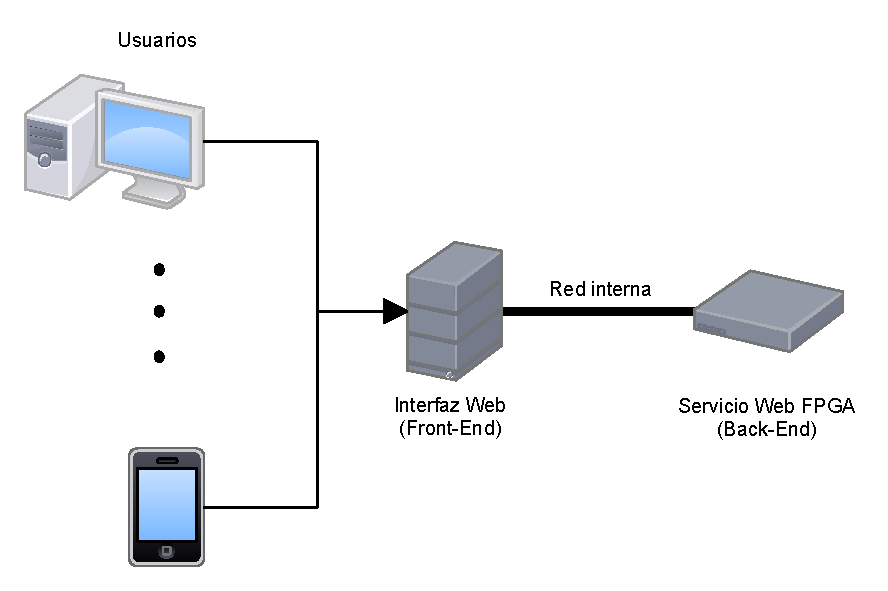
\includegraphics[width=0.9\linewidth]{arquitectura}
  \end{figure}
\end{frame}

% Stack de tecnologías
\begin{frame}{Stack tecnológico}
  \begin{itemize}
    \item\alert<+>{Back-End}
    \begin{itemize}
      \item JavaScript
      \item node.js
      \item express, async, nodemon
    \end{itemize}
    \item\alert<+>{Front-End}
    \begin{itemize}
      \item PHP (HTML, JavaScript, CSS)
      \item Framework propio
      \item Bootstrap, jQuery
    \end{itemize}
  \end{itemize}
\end{frame}

% Back-End
\begin{frame}{Back-End - Servicio Web FPGA}
  \begin{itemize}[<alert@+>]
    \item Formalizar y exponer la funcionalidad de la FPGA
    \item Permite conocer el estado de la misma y de aspectos relacionados
    \item Implementación REST-like
  \end{itemize}
  \begin{figure}
    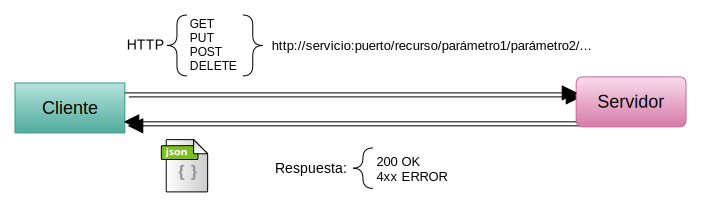
\includegraphics[width=\linewidth]{fpga_rest}
  \end{figure}
\end{frame}

\begin{frame}{Back-End - Arquitectura interna}
  \begin{figure}
    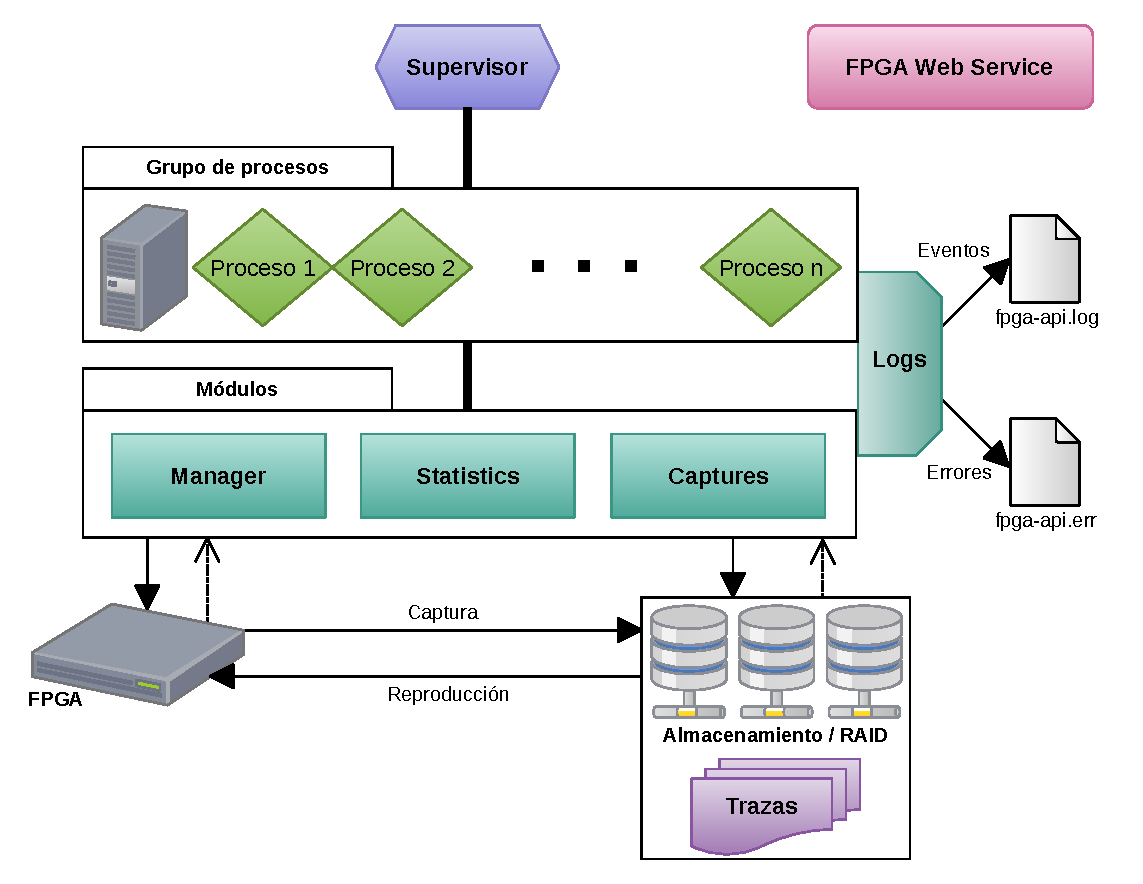
\includegraphics[width=0.85\linewidth]{fpga}
  \end{figure}
\end{frame}

\begin{frame}{Back-End - FSM Estado FPGA}
  \begin{itemize}
    \item Formaliza el estado de la FPGA de forma no persistente
  \end{itemize}
  \begin{figure}
    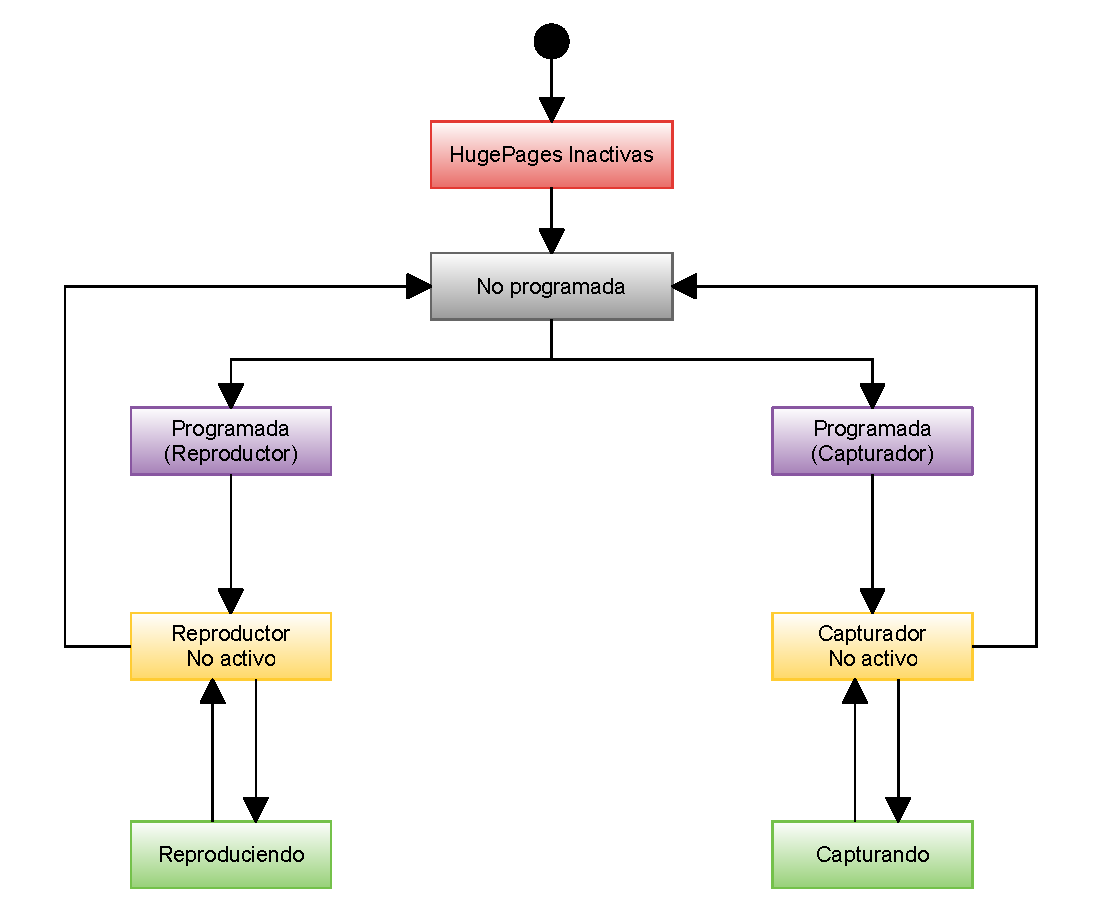
\includegraphics[width=0.65\linewidth, valign=t]{fpga_estado}
    \hfill
    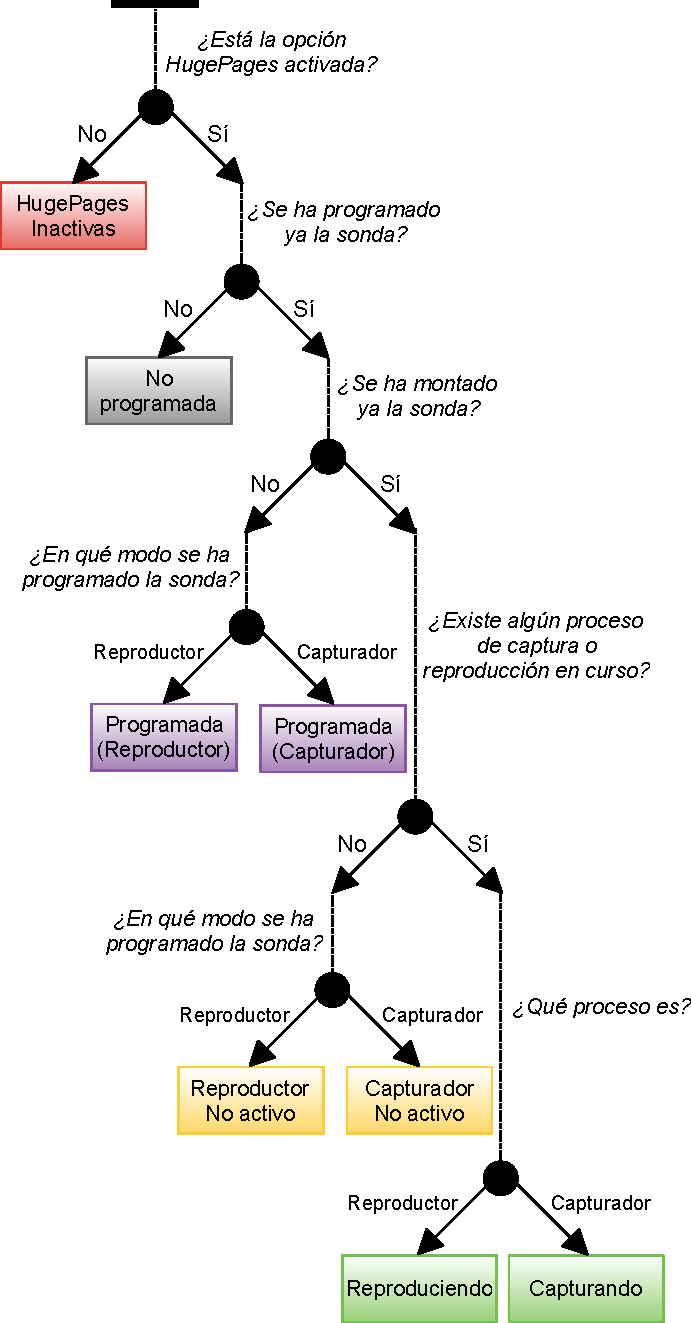
\includegraphics[height=0.7\textheight, valign=t]{arbol_decision_vertical}
  \end{figure}
\end{frame}

\begin{frame}{Back-End - API REST-like}
  \begin{itemize}
    \item API REST-like - Métodos accesibles por HTTP
  \end{itemize}
  \begin{figure}
    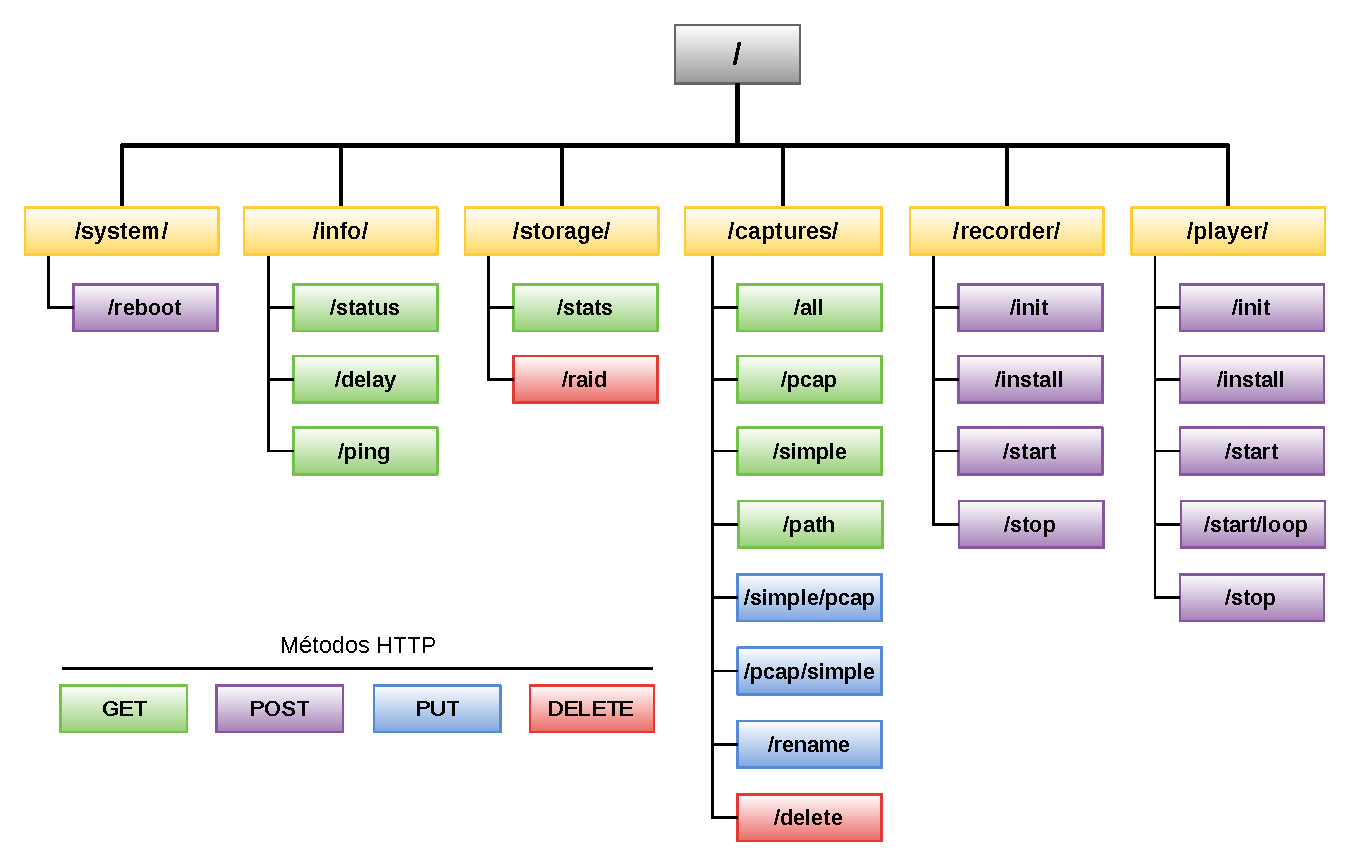
\includegraphics[width=0.9\linewidth]{arbol_metodos}
  \end{figure}
\end{frame}

% Front-End
\begin{frame}{Front-End - Framework - Arquitectura interna}
  \begin{itemize}
    \item Framework propio - únicamente la funcionalidad necesaria
  \end{itemize}
  \begin{figure}
    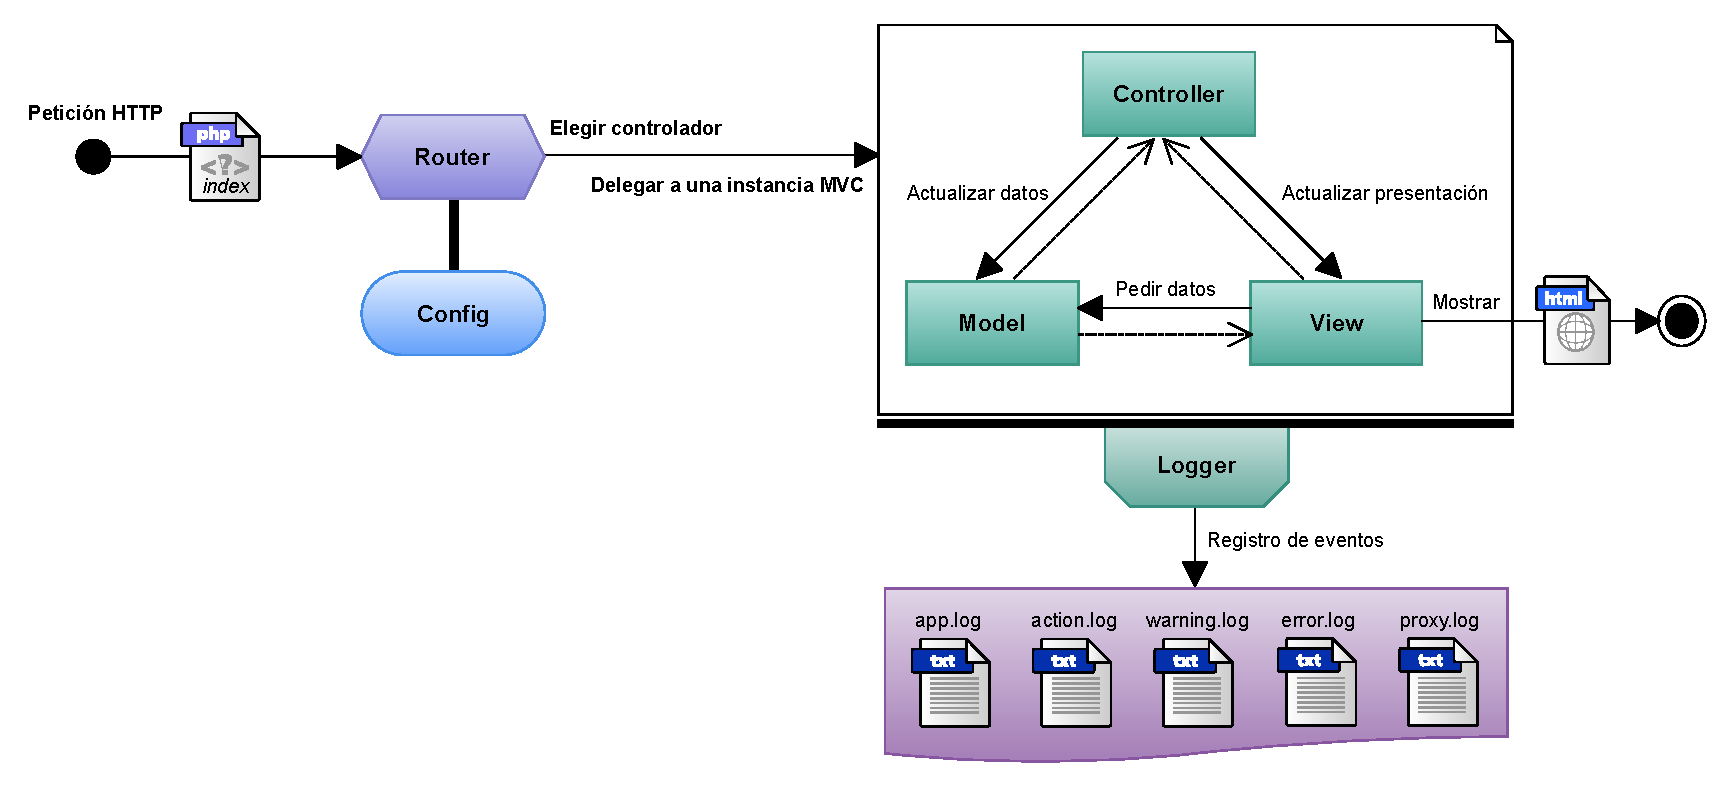
\includegraphics[width=\linewidth]{framework}
  \end{figure}
\end{frame}

\begin{frame}{Front-End - Framework - Router}
  \begin{itemize}
    \item Carga el módulo/método correspondiente para cada petición HTTP
  \end{itemize}
  \begin{figure}
    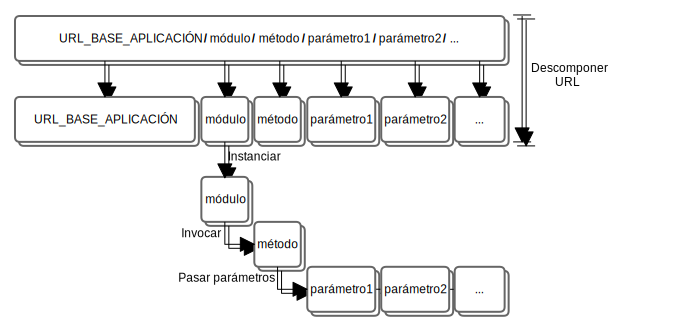
\includegraphics[width=\linewidth]{router}
  \end{figure}
\end{frame}

\begin{frame}{Front-End - Framework - Proxy}
  \begin{itemize}
    \item Comunicación con el Servicio Web FPGA
  \end{itemize}
  \begin{figure}
    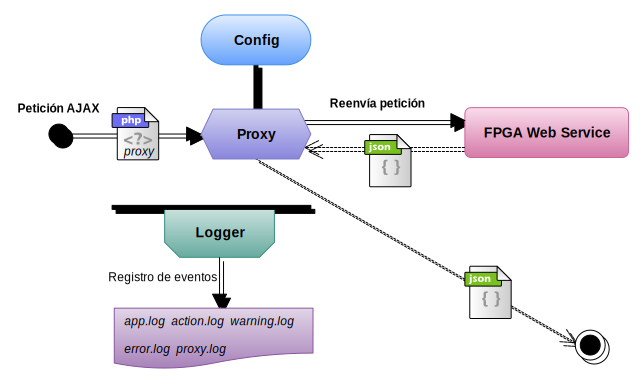
\includegraphics[width=\linewidth]{proxy}
  \end{figure}
\end{frame}

\begin{frame}{Front-End - Diseño - Capturas}
  \begin{figure}
    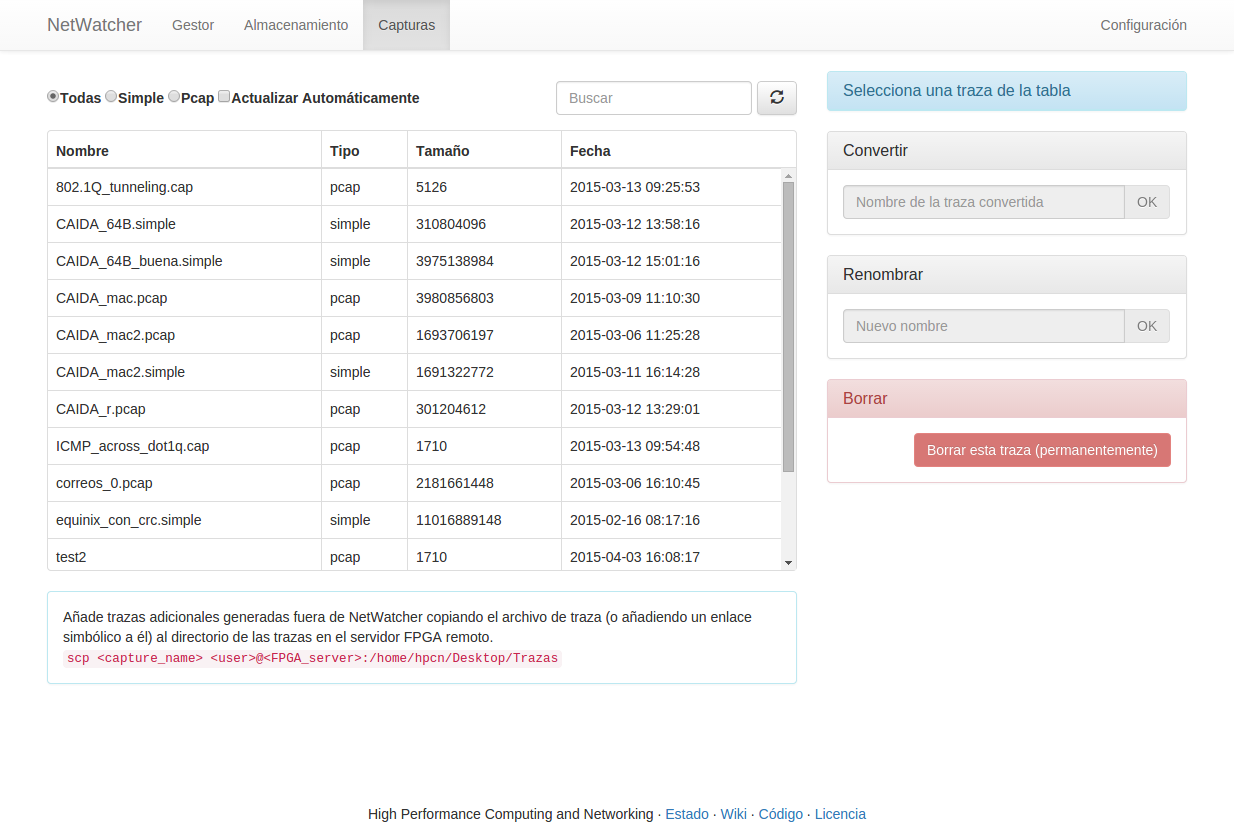
\includegraphics[width=\linewidth]{capturas}
  \end{figure}
\end{frame}

\begin{frame}{Front-End - Diseño - Gestor capturar}
  \begin{figure}
    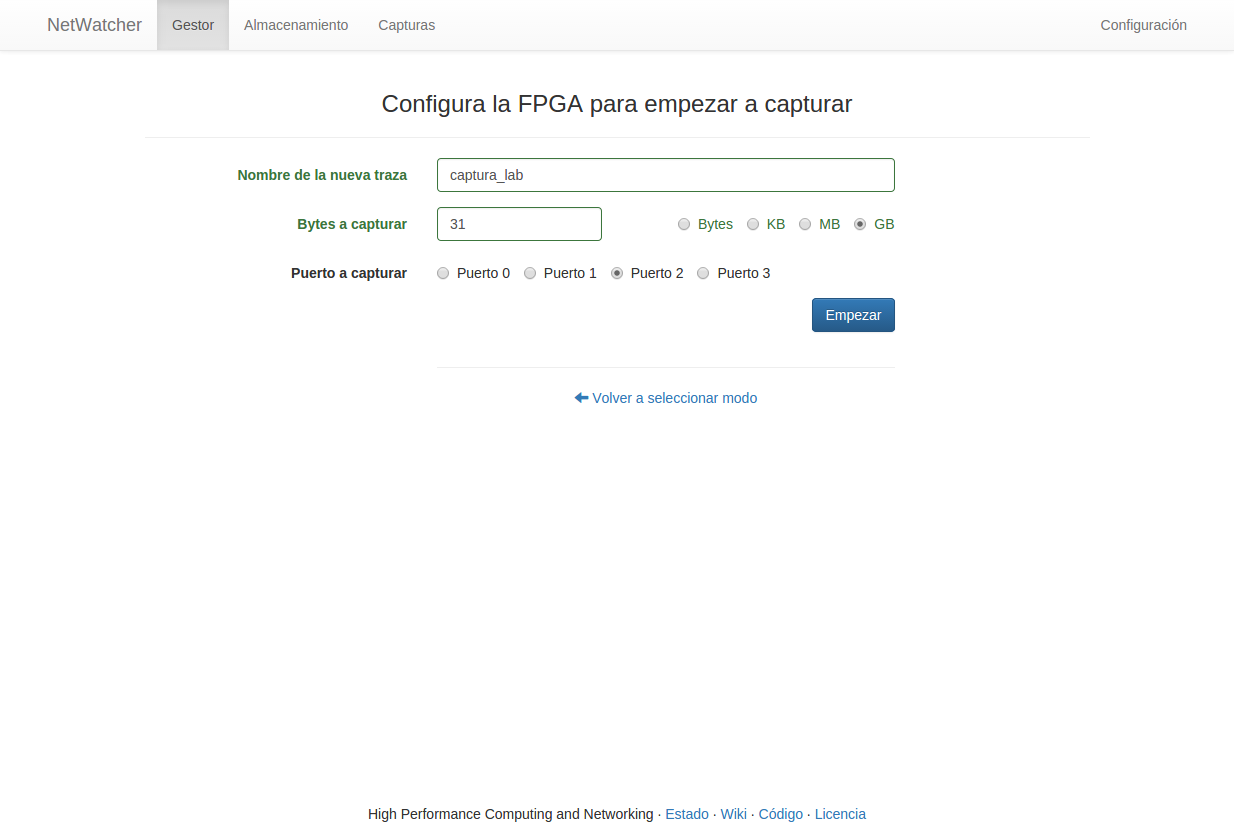
\includegraphics[width=\linewidth]{gestor_capturar}
  \end{figure}
\end{frame}

\begin{frame}{Front-End - Diseño - Estado}
  \begin{itemize}
    \item Diseño \textit{responsive} - adaptado a cada dispositivo
  \end{itemize}
  \begin{figure}
    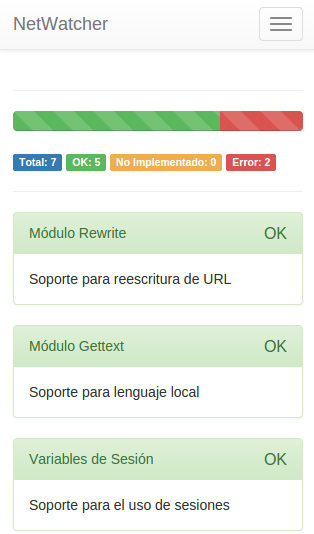
\includegraphics[width=0.3\linewidth]{estado_movil}
  \end{figure}
\end{frame}


% Conclusiones
\section{Conclusiones}

\begin{frame}{Conclusiones}
  \begin{itemize}
    \item Gestión del sistema completo mediante una interfaz web
    \begin{itemize}
      \item Control de la FPGA de forma intuitiva
    \end{itemize}
    \item Trabajo extensible a otras sondas de red
    \begin{itemize}
      \item Arquitectura base
      \item Módulos independientes del modelo de sonda
      \begin{itemize}
        \item Clasificación y conversión de trazas
        \item Almacenamiento
        \item Velocidad del disco
        \item Estado global del sistema
      \end{itemize}
    \end{itemize}
    \item Se registra el uso tanto del Back-End como del Front-End
    \item Se cumplen todos los objetivos propuestos
  \end{itemize}
\end{frame}

\begin{frame}{Contribuciones}
  \begin{itemize}
    \item Proyecto europeo de federación Fed4FIRE
    \begin{itemize}
      \item Desarrollado de forma paralela al TFG
      \item Back-End utilizado en la integración del testbed de la FPGA
      \begin{itemize}
        \item Permite exponer la funcionalidad de la sonda de red sin que el usuario tenga acceso al servidor al que está conectada
      \end{itemize}
    \end{itemize}
    \item The Open Source Network Tester
    \begin{itemize}
      \item Posible incorporación de la interfaz desarrollada
    \end{itemize}
    \item Proyecto disponible en GitHub
    \begin{itemize}
      \item Liberado bajo licencia MIT
      \item Documentación extensiva
    \end{itemize}
  \end{itemize}
\end{frame}


% Líneas de Trabajo Futuro
\section{Líneas de Trabajo Futuro}

\begin{frame}{Líneas de Trabajo Futuro}
  \begin{itemize}[<alert@+>]
    \item Extensión a más sondas de red
    \item Módulo de autenticación
    \item Soporte a tipos de trazas
    \item Registro de estadísticas adicionales
    \item Interfaz en otros idiomas
  \end{itemize}
\end{frame}


% Preguntas
\plain{Preguntas}

\end{document}
